% Preambulo donde están los paquetes que tienen los comandos que se usan en el código.
\documentclass[12pt, a4paper, spanish, twoside]{article}
% Sacar draft para que aparezcan las imagenes.
% Opciones: 12pt, 10pt, 11pt, landscape, twocolumn, fleqn, leqno...
% Opciones de clase: article, report, letter, beamer...

% Paquetes:
% =========
\usepackage[headheight=110pt, top = 2cm, bottom = 2cm, left=1cm, right=1cm]{geometry} %modifico márgenes
\usepackage[T1]{fontenc} % tildes
\usepackage[utf8]{inputenc} % Para poder escribir con tildes en el editor.
\usepackage[english]{babel} % Para cortar las palabras en silabas, creo.
\usepackage[ddmmyy]{datetime}
\usepackage{amsmath} % Soporte de mathmatics
\usepackage{mathtools} % Más herramientas para matemáctica
\usepackage{amssymb} % fuentes de mathmatics
\usepackage{array} % Para tablas y eso
\usepackage[dvipsnames]{xcolor} % Para colorear el texto: black, blue, brown, cyan, darkgray, gray, green, lightgray, lime, magenta, olive, orange, pink, purple, red, teal, violet, white, yellow.
\usepackage{enumitem} % Cambiar labels y más flexibilidad para el enumerate
\usepackage{multicol} 
\usepackage{tikz} % para graficar
\usepackage{cancel} % cancelar fórmulas
\usepackage{titlesec} % para editar titulos y hacer secciones con formato a medida
\usepackage{ulem}
\usepackage{centernot} % tacha cosas
\usepackage{bbding} % símbolos de donde uso FiveStar
\usepackage{skull} % símbolos de donde uso Skull
\usepackage{soul} % Para tachar texto en text y math mode
\usepackage{polynom} % para división de polinomios y mcd
\usepackage{fontawesome5} % fuentes "extras"
\usepackage{venndiagram} % Para los diagramas de Venn
\usepackage{qrcode} % genera código qr
%\usepackage{listings} % Escribir código

%\usepackage{algorithm}
%\usepackage{algpseudocode}
%\usepackage{algorithmicx}

\usepackage{fancyhdr} % Encabezados y pie de páginas
% \usepackage{lipsum} % dummy text
% \usepackage{caption} % Configuracion de figuras y tablas



% para hacer los graficos tipo grafos
\usetikzlibrary{shapes,arrows.meta, chains, matrix, calc, trees, positioning, fit}
\usetikzlibrary{external,decorations.pathreplacing,angles,quotes}

% En general quiero que este paquete sea el último en importarse
\usepackage{hyperref} % para que haya links navegables en el PDF
\hypersetup{
    colorlinks=true,
    linkcolor=blue,
    %filecolor=magenta,
    urlcolor=OliveGreen!90!black,
    pdftitle={Álgebra I - Resuelta, sueltísima},
    pdfauthor={Por los alumnos y exalumnos de Álgebra I}
    }
\urlstyle{same}

\setlength{\parindent}{0pt} % Para que no haya indentación en las nuevas líneas.

%% Info SOCIAL
\def\dirRepo{https://github.com/nad-garraz/algebraUno}
\def\dirTelegram{https://t.me/+1znt2GV1i8cwMTNh}
\newcommand{\dirGuia}[1]{\dirRepo/blob/main/#1-guia/#1-sol.pdf}


% Gráficos fuera del documento para que el código quede un poco más limpio
%3
\def\tresiiiUno{
	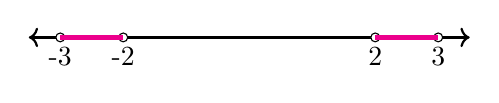
\begin{tikzpicture}[scale=0.8, baseline=0]
		% Number line
		\draw[thick, <->,] (-3.5,0) -- (3.5,0);
		% Interval
		\draw[fill=white] (2,0) circle (2pt);
		\draw[fill=white] (3,0) circle (2pt);
		\draw[fill=white] (-2,0) circle (2pt);
		\draw[fill=white] (-3,0) circle (2pt);
		\draw[-, magenta, ultra thick] (2,0) -- (3,0);
		\draw[-, magenta, ultra thick] (-2,0) -- (-3,0);
		\node at (2,-0.3) {2};
		\node at (3,-0.3) {3};
		\node at (-2,-0.3) {-2};
		\node at (-3,-0.3) {-3};
	\end{tikzpicture}
}
\def\tresiiiDos{
	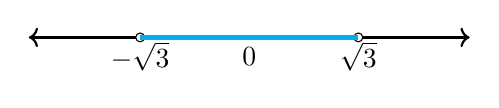
\begin{tikzpicture}[scale=0.8, baseline=0]
		% Number line
		\draw[thick, <->,] (-3.5,0) -- (3.5,0);
		% Interval
		\draw[fill=white] (1.732,0) circle (2pt);
		\draw[fill=white] (-1.732,0) circle (2pt);
		\draw[-, cyan, ultra thick] (1.732,0) -- (-1.732,0);
		\node at (1.732,-0.3) {$\sqrt{3}$};
		\node at (-1.732,-0.3) {$-\sqrt{3}$};
		\node at (0,-0.3) {0};
	\end{tikzpicture}
}

%12
\def\doceiA{
	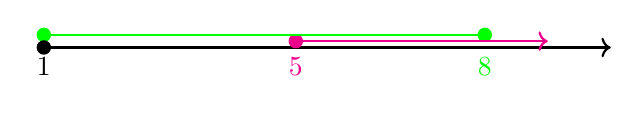
\begin{tikzpicture}[scale=0.8, baseline=0]
		% Number line
		\draw[thick, ->,] (1,0) -- (10,0);
		% Interval
		\draw[fill=magenta, color=magenta] (5,0.1) circle (3pt);
		\draw[fill=green, color=green] (8,0.2) circle (3pt);
		\draw[fill=green, color=green] (1,0.2) circle (3pt);
		\draw[fill=black] (1,0) circle (3pt);
		\draw[-, green, thick] (1,0.2) -- (8,0.2);
		\draw[->, magenta, thick] (5,0.1) -- (9,0.1);
		\node at (1,-0.3) {1};
		\node [color=magenta]at (5,-0.3) {5};
		\node[color=green] at (8,-0.3) {8};
	\end{tikzpicture}
}
\def\doceiiA{
	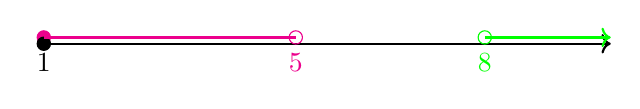
\begin{tikzpicture}[scale=0.8, baseline=0]
		% Number line
		\draw[thick, ->,] (1,0) -- (10,0);
		% Interval
		\draw[color=magenta] (5,0.1) circle (3pt);
		\draw[color=green] (8,0.1) circle (3pt);
		\draw[fill=magenta, color=magenta] (1,0.1) circle (3pt);
		\draw[fill=black] (1,0) circle (3pt);
		\draw[-, magenta, thick] (1,0.1) -- (5,0.1);
		\draw[->, green, thick] (8,0.1) -- (10,0.1);
		\node at (1,-0.3) {1};
		\node [color=magenta]at (5,-0.3) {5};
		\node[color=green] at (8,-0.3) {8};
	\end{tikzpicture}
}

\def\doceiiE{
	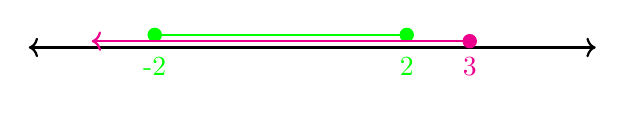
\begin{tikzpicture}[scale=0.8, baseline=0]
		% Number line
		\draw[thick, <->,] (-4,0) -- (5,0);
		% Interval
		\draw[fill=magenta, color=magenta] (3,0.1) circle (3pt);
		\draw[fill=green, color=green] (2,0.2) circle (3pt);
		\draw[fill=green, color=green] (-2,0.2) circle (3pt);
		\draw[<-, magenta, thick] (-3,0.1) -- (3,0.1);
		\draw[-, green, thick] (-2,0.2) -- (2,0.2);
		\node [color=magenta] at (3,-0.3) {3};
		\node[color=green] at (2,-0.3) {2};
		\node[color=green] at (-2,-0.3) {-2};
	\end{tikzpicture}
}

\def\doceiiicero{
	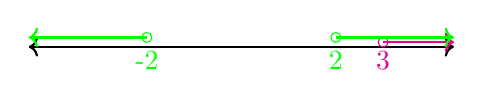
\begin{tikzpicture}[scale=0.6, baseline=0]
		% Number line
		\draw[thick, <->,] (-4.5,0) -- (4.5,0);
		% Interval
		\draw[color=magenta] (3,0.1) circle (3pt);
		\draw[color=green] (2,0.2) circle (3pt);
		\draw[color=green] (-2,0.2) circle (3pt);

		\draw[->, magenta, thick] (3,0.1) -- (4.5,0.1);
		\draw[<-, green, thick] (-4.5,0.2) -- (-2,0.2);
		\draw[->, green, thick] (2,0.2) -- (4.5,0.2);

		\node[color=magenta] at (3,-0.3) {3};
		\node[color=green] at (2,-0.3) {2};
		\node[color=green] at (-2,-0.3) {-2};
	\end{tikzpicture}
}

\def\doceiiiuno{
	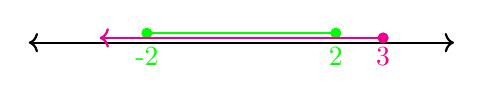
\begin{tikzpicture}[scale=0.6, baseline=0]
		% Number line
		\draw[thick, <->,] (-4.5,0) -- (4.5,0);
		% Interval
		\draw[fill=magenta, color=magenta] (3,0.1) circle (3pt);
		\draw[fill=green, color=green] (2,0.2) circle (3pt);
		\draw[fill=green, color=green] (-2,0.2) circle (3pt);

		\draw[<-, magenta, thick] (-3,0.1) -- (3,0.1);
		\draw[-, green, thick] (-2,0.2) -- (2,0.2);

		\node[color=magenta] at (3,-0.3) {3};
		\node[color=green] at (2,-0.3) {2};
		\node[color=green] at (-2,-0.3) {-2};
	\end{tikzpicture}
}

\def\doceiiidos{
	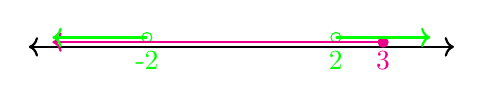
\begin{tikzpicture}[scale=0.6, baseline=0]
		% Number line
		\draw[thick, <->,] (-4.5,0) -- (4.5,0);
		% Interval
		\draw[fill=magenta, color=magenta] (3,0.1) circle (3pt);
		\draw[color=green] (2,0.2) circle (3pt);
		\draw[color=green] (-2,0.2) circle (3pt);

		\draw[<-, magenta, thick] (-4,0.1) -- (3,0.1);
		\draw[<-, green, thick] (-4,0.2) -- (-2,0.2);
		\draw[->, green, thick] (2,0.2) -- (4,0.2);

		\node[color=magenta] at (3,-0.3) {3};
		\node[color=green] at (2,-0.3) {2};
		\node[color=green] at (-2,-0.3) {-2};
	\end{tikzpicture}
}

\def\doceiiitres{
	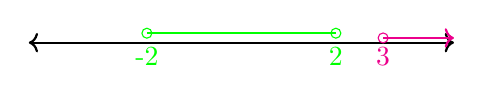
\begin{tikzpicture}[scale=0.6, baseline=0]
		% Number line
		\draw[thick, <->,] (-4.5,0) -- (4.5,0);
		% Interval
		\draw[color=magenta] (3,0.1) circle (3pt);
		\draw[color=green] (2,0.2) circle (3pt);
		\draw[color=green] (-2,0.2) circle (3pt);

		\draw[->, magenta, thick] (3,0.1) -- (4.5,0.1);
		\draw[-, green, thick] (-2,0.2) -- (2,0.2);

		\node[color=magenta] at (3,-0.3) {3};
		\node[color=green] at (2,-0.3) {2};
		\node[color=green] at (-2,-0.3) {-2};
	\end{tikzpicture}
}

% 17
\def\diecisietei{
	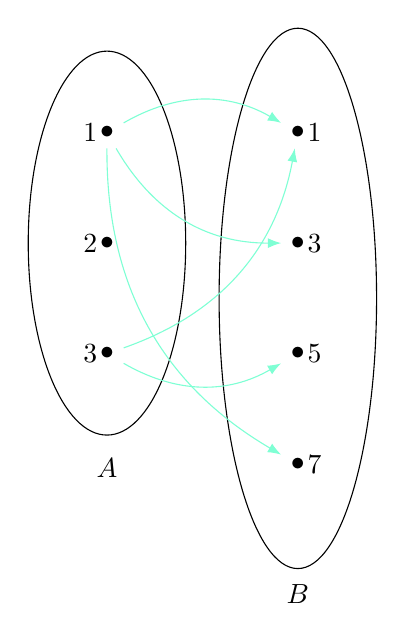
\begin{tikzpicture}[scale=0.5, >=Latex, draw=Aquamarine]
		%A vértices
		\node (1a) {$\bullet$};
		\node[] at (1a.west) {1};
		\node[below=of 1a] (2a) {$\bullet$};
		\node[] at (2a.west) {2};
		\node[below=of 2a] (3a) {$\bullet$};
		\node[] at (3a.west) {3};
		\node[shape=ellipse, draw, black, minimum size=2cm,fit={(1a) (3a)}] {};

		%B vértices
		\node[right=2cm of 1a] (1b) {$\bullet$};
		\node[] at (1b.east) {1};
		\node[below=of 1b] (3b) {$\bullet$};
		\node[] at (3b.east) {3};
		\node[below=of 3b] (5b) {$\bullet$};
		\node[] at (5b.east) {5};
		\node[below=of 5b] (7b) {$\bullet$};
		\node[] at (7b.east) {7};
		\node[shape=ellipse, draw, black, minimum size=2cm,fit={(1b) (7b)}] {};

		% Elipses
		\node[below=1cm of 3a] {$A$};
		\node[below=1.2cm of 7b] {$B$};

		% Aristas
		\draw[->, bend left] (1a) to (1b);
		\draw[->, bend right] (1a) to (3b);
		\draw[->, bend right] (1a) to (7b);
		\draw[->, bend right] (3a) to (1b);
		\draw[->, bend right] (3a) to (5b);
	\end{tikzpicture}
}

%19
\def\diecinuevei{
	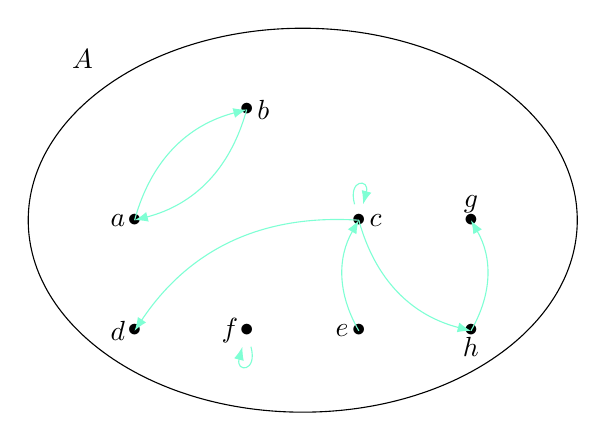
\begin{tikzpicture}[scale=0.5, baseline=0, >=Latex, draw=Aquamarine]

		\node[] (a) {$\bullet$};
		\node[] at (a.west) {$a$};

		\node[above right= of a] (b) {$\bullet$};
		\node[] at (b.east) {$b$};

		\node[below right= of b] (c) {$\bullet$};
		\node[] at (c.east) {$c$};

		\node[below= of a] (d) {$\bullet$};
		\node[] at (d.west) {$d$};

		\node[below= of c] (e) {$\bullet$};
		\node[] at (e.west) {$e$};

		\node[right= of d] (f) {$\bullet$};
		\node[] at (f.west) {$f$};

		\node[right= of c] (g) {$\bullet$};
		\node[] at (g.north) {$g$};

		\node[below= of g] (h) {$\bullet$};
		\node[] at (h.south) {$h$};

		% Universo
		\node[shape=ellipse, draw, black, fit={ (b) (d) (g) (e)}] (universo) {};
		\node[above left = 0.1cm of universo] {$A$};

		% Aristas
		\draw[->, bend left] (a.center) to (b.center);
		\draw[->, bend left] (b.center) to (a.center);
		\draw[->, bend right] (c.center) to (d.center);
		\draw[->, loop above] (c) to (c);
		\draw[->, loop below ] (f) to (f);
		\draw[->, bend right] (c.center) to (h.center);
		\draw[->, bend left] (e.center) to (c.center);
		\draw[->, bend right] (h.center) to (g.center);
	\end{tikzpicture}
}

% 19 ii
\def\diecinueveiv{
	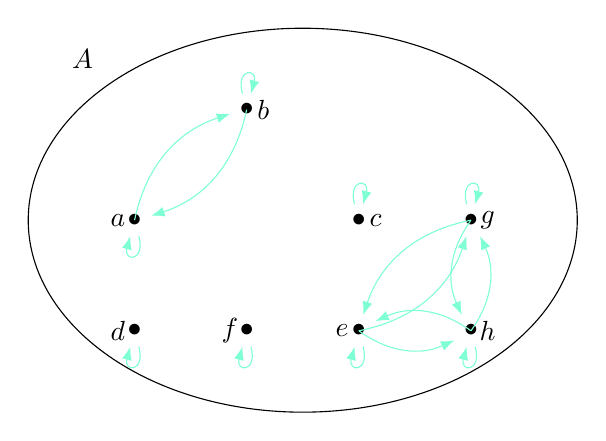
\begin{tikzpicture}[scale=0.5, baseline=0, >=Latex, draw=Aquamarine]

		\node[] (a) {$\bullet$};
		\node[] at (a.west) {$a$};

		\node[above right= of a] (b) {$\bullet$};
		\node[] at (b.east) {$b$};

		\node[below right= of b] (c) {$\bullet$};
		\node[] at (c.east) {$c$};

		\node[below= of a] (d) {$\bullet$};
		\node[] at (d.west) {$d$};

		\node[below= of c] (e) {$\bullet$};
		\node[] at (e.west) {$e$};

		\node[right= of d] (f) {$\bullet$};
		\node[] at (f.west) {$f$};

		\node[right= of c] (g) {$\bullet$};
		\node[] at (g.east) {$g$};

		\node[below= of g] (h) {$\bullet$};
		\node[] at (h.east) {$h$};

		% Universo
		\node[shape=ellipse, draw, black, fit={ (b) (d) (g) (e)}] (universo) {};
		\node[above left = 0.1cm of universo] {$A$};

		% Aristas
		\draw[->, loop below] (a) to (a);
		\draw[->, loop above ] (b) to (b);
		\draw[->, loop above] (c) to (c);
		\draw[->, loop below ] (d) to (d);
		\draw[->, loop below] (e) to (e);
		\draw[->, loop below] (f) to (f);
		\draw[->, loop above] (g) to (g);
		\draw[->, loop below ] (h) to (h);

		\draw[->, bend left] (a.center) to (b);
		\draw[->, bend left] (b.center) to (a);

		\draw[->, bend right] (e.center) to (h);
		\draw[->, bend right] (e.center) to (g);
		\draw[->, bend right] (h.center) to (g);
		\draw[->, bend right] (h.center) to (e);
		\draw[->, bend right] (g.center) to (h);
		\draw[->, bend right] (g.center) to (e);
	\end{tikzpicture}
}

%20

\def\veinte{
	\begin{tikzpicture}[scale=0.5, baseline=0, >=Latex, draw=Aquamarine]

		\node[] (1) {$\bullet$};
		\node[] at (1.west) {$1$};

		\node[above right= of 1] (2) {$\bullet$};
		\node[] at (2.east) {$2$};

		\node[below right= of 2] (3) {$\bullet$};
		\node[] at (3.east) {$3$};

		\node[below= of 1] (4) {$\bullet$};
		\node[] at (4.west) {$4$};

		\node[right= of 2] (5) {$\bullet$};
		\node[] at (5.west) {$5$};

		\node[right= of d] (6) {$\bullet$};
		\node[] at (6.east) {$6$};


		% Universo
		\node[shape=ellipse, draw, black, fit={ (1) (2) (3) (4)}] (universo) {};
		\node[above left = 0.1cm of universo] {$A$};

		% Aristas
		\draw[->, loop below] (1) to (1);
		\draw[->, loop above ] (3) to (3);
		\draw[->, loop above] (4) to (4);
		\draw[->, loop below ] (6) to (6);

		\draw[->, bend left] (6.center) to (4);
		\draw[->, bend left] (4.center) to (6);

		\draw[->, bend right] (1.center) to (3);
		\draw[->, bend right] (3.center) to (1);
	\end{tikzpicture}
}

%24
\def\veinticuatro{
	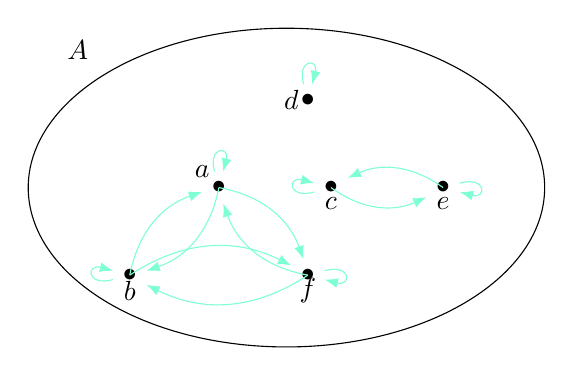
\begin{tikzpicture}[scale=0.5, baseline=0, >=Latex, draw=Aquamarine]

		\node[] (a) {$\bullet$};
		\node[] at (a.north west) {$a$};

		\node[below left = 1cm of a] (b) {$\bullet$};
		\node[] at (b.south) {$b$};

		\node[below right = 1cm of a] (f) {$\bullet$};
		\node[] at (f.south) {$f$};

		\node[above right = 1cm of a] (d) {$\bullet$};
		\node[] at (d.west) {$d$};

		\node[right=1cm of a] (c) {$\bullet$};
		\node[] at (c.south) {$c$};

		\node[right= of c] (e) {$\bullet$};
		\node[] at (e.south) {$e$};


		% Universo
    \node[shape=ellipse, draw, black, fit={ (a) (b) (d) (f) (e)}] (universo) {};
		\node[above left = 0.1cm of universo] {$A$};

		% Aristas
		\draw[->, loop above] (a) to (a);
		\draw[->, loop left ] (b) to (b);
		\draw[->, loop left] (c) to (c);
		\draw[->, loop above ] (d) to (d);
		\draw[->, loop right ] (e) to (e);
		\draw[->, loop right ] (f) to (f);

		\draw[->, bend left] (a.center) to (b);
		\draw[->, bend left] (b.center) to (a);
		\draw[->, bend left] (a.center) to (f);
		\draw[->, bend left] (f.center) to (a);
		\draw[->, bend left] (b.center) to (f);
		\draw[->, bend left] (f.center) to (b);

		\draw[->, bend right] (c.center) to (e);
		\draw[->, bend right] (e.center) to (c);
	\end{tikzpicture}
}

%25
\def\veintisiete{
	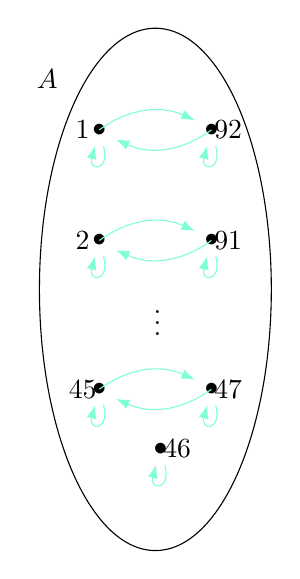
\begin{tikzpicture}[scale=0.5, baseline=0, >=Latex, draw=Aquamarine]

		\node[] (1) {$\bullet$};
		\node[] at (1.west) {$1$};

		\node[right = of 1] (92) {$\bullet$};
		\node[] at (92.east) {$92$};

		\node[below = of 1] (2) {$\bullet$};
		\node[] at (2.west) {$2$};

		\node[right = of 2] (91) {$\bullet$};
		\node[] at (91.east) {$91$};

		\node[below right = .5 of 2] (puntos) {$\vdots$};

		\node[below left = .5 of puntos] (45) {$\bullet$};
		\node[] at (45.west) {$45$};

		\node[right = of 45] (47) {$\bullet$};
		\node[] at (47.east) {$47$};


		\node[below right =.5 of 45] (46) {$\bullet$};
		\node[] at (46.east) {$46$};


		% Universo
    \node[shape=ellipse, draw, black, fit={ (1) (92) (45) (47) (46)}] (universo) {};
		\node[above left = 0.1cm of universo] {$A$};

		% Aristas
		\draw[->, loop below] (1) to (1);
		\draw[->, loop below ] (92) to (92);

		\draw[->, loop below] (2) to (2);
		\draw[->, loop below ] (91) to (91);

		\draw[->, loop below] (45) to (45);
		\draw[->, loop below ] (47) to (47);

		\draw[->, loop below ] (46) to (46);

		\draw[->, bend left] (1.center) to (92);
		\draw[->, bend left] (92.center) to (1);
		\draw[->, bend left] (2.center) to (91);
		\draw[->, bend left] (91.center) to (2);
		\draw[->, bend left] (45.center) to (47);
		\draw[->, bend left] (47.center) to (45);
	\end{tikzpicture}
}
 

\begin{document}

% Info para armar título.
\title{Práctica 1 de álgebra 1} % título
% === Buscar forma más agradable de presentar a los que contribuyan
\author{La comunidad algebraica} % autor

\date{last update: \today} % Cambiar de ser necesario
\maketitle  % Para que aprezca el título en el documento

% Archivo con notas teóricas
\hypertarget{teoria-1:basicos-conjuntos}\textit{Básicos sobre conjuntos y coso: }
\begin{itemize}[label={\tiny\faIcon{smile}}]
  \item \textit{ Las uniones e intersecciones de conjuntos conmutan:}
        $$
          \begin{array}{c}
            A \union B = B \union A \\
            A \inter B = B \inter A
          \end{array}
        $$

  \item
        \textit{De Morgan Law's: }
        $$
          \begin{array}{c}
            (A \union B)^c = A^c \inter B^c \to \text{De Morgan 1} \\
            (A \inter B)^c = A^c \union B^c \to \text{De Morgan 2}
          \end{array}
        $$

  \item \textit{Distribución de la intersección en una unión y alverre: }
        $$
          \begin{array}{c}
            A \yellow{\inter} (B \union C) = (A \yellow{\inter} B) \union (A \yellow{\inter} C) \\
            A \cyan{\union} (B \inter C) = (A \cyan{\union} B) \inter (A \cyan{\union} C)
          \end{array}
        $$
        \begin{center}
          \begin{venndiagram3sets}[shade=orange!30!white, showframe = false,hgap=0, vgap=0, overlap = 1.1cm]
            \fillACapB
            \fillACapC
          \end{venndiagram3sets}
          \begin{venndiagram3sets}[shade=cyan, showframe = false,hgap=0, vgap=0, overlap = 1.1cm]
            \fillA
            \fillBCapC
          \end{venndiagram3sets}
        \end{center}

  \item \textit{Diferencias en sus varios colores, sabores y notaciones: }
        $$
          \begin{array}{c}
            A - B
            \Sii{idem}[notación]
            A \diferencia B
            \Sii{idem}[notación]
            A \inter B^c
          \end{array}
          \
        $$
        \begin{center}
          \begin{venndiagram2sets}[shade=gray!20!white, showframe = false,hgap=0, vgap=0, overlap = 1.1cm]
            \fillANotB
          \end{venndiagram2sets}
        \end{center}

  \item \textit{Diferencia simétrica: }\par
        $$
          A \triangle B =
          \llave{lcl}{
            (A - B)        & \union      & (B - A)                                                     \\
            (A \union B)   & \inter      & (A \inter B)^c                                              \\
            (A \union B)   & \diferencia & (A \inter B)  \to \text{mi favorita \faIcon{meh}} \\
            (A \inter B^c) & \union      & (B \inter A^c)
          }
        $$

        \begin{center}
          \begin{venndiagram2sets}[shade=gray!20!white, showframe = false,hgap=0, vgap=0, overlap = 1.1cm]
            \fillANotB
            \fillBNotA
          \end{venndiagram2sets}
        \end{center}

  \item \textit{Complemento:}\par
        $$
          A^c = \set{x \en \universo \talque x \notin A}
        $$

  \item \hypertarget{teoria-1:tablasDeVerdad}{\textit{Tablas de verdad: }}
        %%%MACRO
        \def\subconjuntoYequivalente{
          \begin{array}{|c|}
            A \subseteq B \\
            \hline
            A^c \union B
          \end{array}
        }
        %%%END MACRO

        En las tablas de verdad que un elemento esté en un conjunto, $x \en A$ es equivalente a decir que la proposición $A$ es verdadera.
        En mi cabeza es más fácil recordar las tablas en conjuntos que en ... lo otro.
        \[
          \begin{array}{|c|c|c|c|c|c|c|c|}
            \hline
            x \en A & x \en B & x \en A^c & x \en A \inter B & x \en A \union B & x \en \subconjuntoYequivalente & x \en A \triangle B & A - B \\
            \hline
            V       & V       & F         & V                & V                & V                              & F                   & F     \\
            V       & F       & F         & F                & V                & F                              & V                   & V     \\
            F       & V       & V         & F                & V                & V                              & V                   & F     \\
            F       & F       & V         & F                & F                & V                              & F                   & F     \\
            \hline
          \end{array}
        \]

        Cuando para probar $p \entonces q$ se prueba en su lugar $\neg q \entonces \neg p$ se dice que es
        una \textit{demostración
          por contrarrecíproco}.\par
        Cuando para probar $p \entonces q$ se prueba en su lugar $p \land \neg q$ para llegar así
        a una contradicción, se dice que es una demostración por reducción al absurdo.

  \item \hypertarget{teoria-1:relaciones}{\textit{Relaciones $\relacion$:}}\par
        \begin{itemize}[label=\tiny\faIcon{yin-yang}]
          \item
                \textit{Definición de relación: }\par
                Sean $A$ y $B$ conjuntos. Una relación $\relacion$ de $A$ en $B$ es un suconjunto
                cualquiera $\relacion$ del producto cartesiano $A \times B$. Es decir $\relacion$ es una relación
                de $A$ en $B$ si $\relacion \en \partes(A \times B)$.
          \item
                \textit{Definición de relación en un conjunto: }\par
                Sea $A$ un conjunto. Se dice que $\relacion$ en $A$ cuando $\relacion \subseteq A \times A$.
        \end{itemize}

  \item \hypertarget{teoria-1:prop-relaciones}{\textit{Propiedades destacables de una $\relacion$:}}\par
        \begin{enumerate}[label=\tiny\faIcon{poop}]
          \item  \textit{Reflexiva}: $(x, x) \en \relacion \paratodo x \en A$ o $x \relacion x.\, \paratodo x \en A$. Gráficamente,
                cada elemento tiene que tener un bucle.
                \begin{tikzpicture}[baseline=0, >=Latex, draw=Aquamarine]
                  \node[](a) {$\bullet$} edge [in=0,out=90,loop] ();
                  \node[] at (a.west) {$x$};
                \end{tikzpicture}

          \item  \textit{Simétrica}: $(x, y) \en \relacion$, entonces el par $(y, x) \en \relacion$,
                también si $\paratodo x, y \en A, x\relacion y \entonces y \relacion x$.
                Gráficamente tiene que haber un ida y vuelta en cada elemento de la relación.
                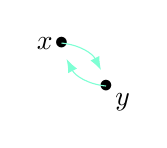
\begin{tikzpicture}[baseline=-10, >=Latex, draw=Aquamarine]
                  \node[] (x) {$\bullet$};
                  \node[] at (x.west) {$x$};
                  \node[below right =0.2 of x] (y) {$\bullet$};
                  \node[] at (y.south east) {$y$};
                  \draw[->, bend left=1cm] (x.center) to (y);
                  \draw[->, bend left=1cm] (y.center) to (x);
                \end{tikzpicture}

          \item  \textit{Antisimétrica}: $(x, y) \en \relacion$, con $x \distinto y$ entonces el par $(y, x) \notin \relacion$, también se puede pensar
                como $\paratodo x,y \en A, x\relacion y$ e $ y \relacion x \entonces x = y$.
                Gráficamente \textbf{no} tiene que haber ningún ida y vuelta en el gráfico. Solo en una dirección.
                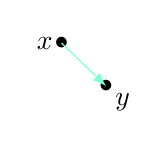
\begin{tikzpicture}[baseline=-10, >=Latex, draw=Aquamarine]
                  \node[] (x) {$\bullet$};
                  \node[] at (x.west) {$x$};
                  \node[below right =0.2 of x] (y) {$\bullet$};
                  \node[] at (y.south east) {$y$};
                  \draw[->] (x.center) to (y.center);
                \end{tikzpicture}

          \item  \textit{Transitiva}: Para toda terna $x, y, z \en A$ tales que $(x, y) \en \relacion$ e $(y,z) \en \relacion$,
                se tiene que $(x, z) \en \relacion$.
                Otra manera sería si $\paratodo x, y, z \en A$, $x \relacion y$ e $y \relacion z \entonces x\relacion z$.
                Gráficamente tiene que haber flecha directa entre las puntas de cualquier camino que vaya por más de dos nodos.
                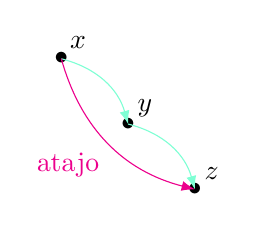
\begin{tikzpicture}[baseline=0, >=Latex, draw=Aquamarine]
                  \node[] (x) {$\bullet$};
                  \node[] at (x.north east) {$x$};
                  \node[below right = 0.6cm of x] (y) {$\bullet$};
                  \node[] at (y.north east) {$y$};
                  \node[below right = 0.6cm of y] (z) {$\bullet$};
                  \node[] at (z.north east) {$z$};

                  \draw[->, bend left] (x.center) to (y.center);
                  \draw[->, bend left] (y.center) to (z.center);
                  \draw[->,magenta, bend right]
                  (x.center)
                  to node[midway,below left] {atajo}
                  (z.center);
                \end{tikzpicture}
        \end{enumerate}
  \item
        \begin{itemize}[label=\tiny\faIcon{poo}]
          \item \textit{Relación de equivalencia}: La relación debe ser reflexiva, simétrica y transitiva.
          \item \textit{Relación de orden}: La relación debe ser reflexiva, antisimétrica y transitiva.
        \end{itemize}

  \item \hypertarget{teoria-1:funciones}{\textit{Funciones $f$:}}

        \begin{itemize}[label=\tiny\faIcon{poo}]
          \item
                Sean $A$ y  $B$ conjuntos, y sea $\relacion$ de $A$ en $B$. Se dice que
                $\relacion$ es una \textit{función} cuando todo elemento $x \en A$ está relacionado con algún
                $y \en B$, y este elemento $y$ es único. Es decir:
                $$\begin{array}{l}
                    \paratodo x \en A, \existe!\, y \en B \talque x \relacion y \\
                    \paratodo x \en A, \existe\, y \en B \talque x\relacion y,
                  \end{array}
                $$
                si  $y, z \en B \text{ son tales que } x \relacion y \ytext x \relacion z \entonces y = z$.

                \begin{itemize}[label=\tiny\faIcon{poop}]
                  \item Dada una función $f:\, A\,(dominio) \to B\,(codominio)$
                        el conjunto \textit{imagen} es:
                        $$
                          \im(f)= \set{y \en B : \existe x \en A \talque f(x) = y}
                        $$

                  \item \textit{Propiedades destacables de una $f$:}
                        \begin{itemize}[label=\tiny\faIcon{spider}]
                          \item \textit{inyectiva:} si $\forall x, x' \en A \text{ tales que } f(x) = f(x')$ se tiene que $ x = x'$
                          \item \textit{sobreyectiva:} si $\forall y \en B, \existe x \en A \text{ tal que } f(x) = y.\: f\text{ es sobreyectiva si } \im(f) = B$
                          \item \textit{biyectiva:} Cuando es \textit{inyectiva} y \textit{sobreyectiva}.
                        \end{itemize}

                  \item \textit{Composición de funciones:}\par
                        $A, B, C$ conjuntos y $f: A \to B \to C,\, g: B \to C$ funciones. Entonces la \textit{composición} de $f$ con $g$, que se nota:
                        $$
                          g \comp f = g(f(x)),\, \paratodo x \en A,
                        $$
                        resulta ser una función $g \comp f$ de $A$ en $C$.

                  \item $f$ es biyectiva cuando $f\inv : B \to A$ es la función que satisface que:\par
                        $$
                          \paratodo y \en B: f\inv(y) = x \sisolosi f(x) = y
                        $$
                \end{itemize}
        \end{itemize}
\end{itemize}


\section*{Ejercicios sueltos que me parecen relevantes}
\subsubsection*{Distributiva}
Probar la propiedad distributiva: $X \inter (Y \union Z) = (X \inter Y) \union (X \inter Z)$\\
Tengo que hacer una doble inclusión:
$\to \begin{cases}
		1) & X \inter (Y \union Z) \subseteq (X \inter Y) \union (X \inter Z) \\
		2) & (X \inter Y) \union (X \inter Z) \subseteq X \inter (Y \union Z)
	\end{cases}$

\begin{enumerate}[label=\arabic*)]
	\item
	      $x \en X \inter (Y \union Z)$ quiere decir que $x \en X$ y
	      $\llaves{c}{
			      x \en Y \\
			      \o      \\
			      x \en Z
		      } $.
	      Por lo tanto $\to
		      \llaves{c}{
			      x \en X \inter Y\\
			      \o \\
			      x \en X \inter Z
		      }$, lo que equivale a $x \en (X \inter Y) \union (X \inter Z)$ \Tilde.\\

	\item
	      Ahora hay que probar la vuelta. Uso razonamiento análogo.
	      $x \en (X \inter Y) \union (X \inter Z)$, por lo que $x \en X$ y
	      $
		      \llaves{c}{
			      x \en X \inter Y \blue{\flecha{dado que}[$Y \subseteq Y \union Z$] x \en X \inter (Y \union Z) }\\
			      \o               \\
			      x \en X \inter Z \blue{\flecha{dado que}[$Z \subseteq Y \union Z$] x \en X \inter (Y \union Z)}
		      }$.
	      Lo que quiere decir \blue{que $x \en X \inter (Y \union Z)$ \Tilde}\\
	      \red{¿Estoy suponiendo cosas que debería demostrar, me estoy salteando pasos?}\\
	      \blue{Para que la solución quede más creíble usé que $S \subseteq S \union T$ fue el dealbreaker. }

\end{enumerate}

\subsubsection*{De Morgan}
Probar la propiedad $(A \inter B)^c = A^c \union B^c$.\\
Tengo que hacer una doble inclusión
$\to \begin{cases}
		1) & (A \inter B)^c \subseteq A^c \union B^c \\
		2) & A^c \union B^c \subseteq (A \inter B)^c
	\end{cases}
$
\begin{enumerate}[label=\arabic*)]
	\item Prueba directa: Si $x \en (A \inter B)^c \entonces x \en A^c \union B^c $\\
	      Por hipótesis $x \en (A \inter B)^c \stacktext{def}{\sisolosi} x \notin A \o x \notin B
		      \entonces x \en A^c \o x \en B^c \entonces x \en A^c \union B^c$\\
	      $\begin{array}{|c|c|c|c|}
			      \hline
			      A & B & A^c \union B^c & (A \inter B)^c \\ \hline
			      V & V & F              & F              \\
			      V & F & V              & V              \\
			      F & V & V              & V              \\
			      F & F & V              & V              \\ \hline
		      \end{array}
	      $

	      \blue{Uso la tabla para ver la definición $x \en (A \inter B)^c \stacktext{def}{\sisolosi} x \notin A \o x \notin B$}

	\item Pruebo por absurdo. Si $\paratodo x \en A^c \union B^c \entonces x \en (A \inter B)^c$\\
	      \green{Supongo} que $ x \notin (A \inter B)^c \stacktext{def}{\sisolosi} x \en (A \inter B) \flecha{por}[hipótesis] x \en A^c \union B^c \to
		      \llaves{c}{
			      x \notin A\\
			      \o \\
			      x \notin B\\
		      }$, por lo que $x \notin A \union B \entonces x \notin A \inter B$ contradiciendo el \green{supuesto}, absurdo. Debe ocurrir que $x \en (A \inter B)^c   $

	      $\begin{array}{|c|c|c|c|c|}
			      \hline
			      A & B & A \inter B & (A \union B) & (A \inter B) \subseteq (A \union B) \\ \hline
			      V & V & V          & V            & V                                   \\
			      V & F & F          & V            & V                                   \\
			      F & V & F          & V            & V                                   \\
			      F & F & F          & F            & V                                   \\ \hline
		      \end{array}
	      $
\end{enumerate}

\newpage
\section*{Ejercicios de la guía}

% Para hacer un input de todos los archivos en la
% carpeta de "ejercicio-1"
\foreach \x in {1,...,30} {
    \input{./ejercicios-1/ej-\x-1}
}

%=============
% Habría que evaluar eliminar o mejorar esta sección de notas

\separador
\separador

\subsection*{Notas random}
\begin{itemize}
	\item Cardinal: cantidad de elementos de un conjunto.
	\item El conjunto $\partes(A)$ tiene $2^n$ el cardinal del conjunto $A$.
	\item Una relación $\relacion$ es un subconjunto de un producto cartesiano.
	\item  Leyes de absorción, obvias pero no tan.
	      $\llave{c}{
			      A \union( A \inter B ) = A\\
			      A \inter ( A \union B ) = A\\
		      }$
	\item probar identidades de conjuntos:
	      \begin{itemize}
		      \item
		            $A = B \to
			            \llave{c}{
				            A \subset B \\
				            B \subset A \\
			            }$
		      \item lógica proposicional
		      \item tabla de verdad
	      \end{itemize}
	\item
\end{itemize}
\end{document}
